\documentclass[
BCOR=5mm,           % Binderkorrektur von 5mm vorsehen
fontsize=11pt,      % Schriftgr��e 11 Punkte
oneside,            % Einseitig
parskip,            % Paragraphen nicht einrücken
headsepline,        % Kopfzeile nach unten durch Linie abgrenzen (scrheadings)
%footbotline,       % Fu�zeile nach unten durch Linie abgrenzen (scrheadings)
plainheadsepline,   % Kopfzeile nach unten durch Linie abgrenzen (scrplain)
plainfootbotline,   % Fu�zeile nach unten durch Linie abgrenzen (scrplain)
%headtopline,       % Kopfzeile nach oben durch Linie abgrenzen (scrheadings)
footsepline,        % Fu�zeile nach oben durch Linie abgrenzen (scrheadings)
plainheadtopline,   % Kopfzeile nach oben durch Linie abgrenzen (scrplain)
plainfootsepline,   % Fu�zeile nach oben durch Linie abgrenzen (scrplain)
]{scrbook}          % Koma-Script Klasse zum setzen eines Buchs


\usepackage{lmodern}

% Die "Standard-Header" f�r deutsche Dokumente
\usepackage[latin1]{inputenc}    % ISO-8859-1 bzw. Latin1 als Encoding
%\usepackage[T1]{fontenc}         % T1 Schriften verwenden (sieht besser aus)
\usepackage[ngerman]{babel}      % Neue deutsche Rechtschreibung 

% "Sch�nere" Schriften einbinden
%\usepackage{mathpazo}            % Serifen-Font mit passendem Math-Font
%\usepackage[scaled=.95]{helvet}  % Serifenloser Font passend zu mathpazo
%\usepackage{courier}             % "Sch�nerer" Festbreiten-Font

% Koma-Script Paket zum setzen vom Kopf- und Fu�zeilen einbinden
%\usepackage{scrpage2}
\usepackage{scrlayer-scrpage}
\RequirePackage{scrlfile}
\ReplacePackage{scrpage2}{scrlayer-scrpage}
\usepackage{substr}

%\pagestyle{scrheadings}
\clearpairofpagestyles
\automark[section]{chapter}

\ohead[\sffamily\scshape\bfseries\large\headmark]
{\sffamily\scshape\bfseries\large\headmark}

\ofoot[\sffamily\thepage]{\sffamily\thepage}

\usepackage{listings}
\lstset{
captionpos=b,                % Beschriftung unterhalb (bottom)
numbers=left,                % Zeilennummern links
frame=trbl,                  % Rahmen zeichnen (top, right, bottom, left)
basicstyle=\small\ttfamily,  % Festbreitenschrift verwenden (small)
language=Java                % Sprache auf Java einstellen
}

\usepackage[ngerman]{translator}

\usepackage[
nonumberlist, % Keine Seitenzahlen anzeigen
acronym,      % Abkürzungsverzeichnis erstellen
toc,          % In Inhaltsverzeichnis aufnehmen
%section       % Verzeichniseintrag als Section
]{glossaries}

% Ein eigenes Verzeichnis definieren (Smbolverzeichnis)
% Das Stichwort- und Abkürzungsverzeichnis wird analog vordefiniert
% Siehe makeindex Aufrufe - Hier werden die Dateiendungen festgelegt
\newglossary[slg]{symbolslist}{syi}{syg}{Symbolverzeichnis}

\makeglossaries


% Paket zum generieren von Blindtext
\usepackage{blindtext}

% Paket zum Einbinden von Bildern
\usepackage{graphicx}

%              
% WORKAROUND, damit lstlistoflistings funktioniert:
% Quelle: http://www.komascript.de/node/477
%
\makeatletter
\@ifundefined{float@listhead}{}{%
    \renewcommand*{\lstlistoflistings}{%
        \begingroup
    	    \if@twocolumn
                \@restonecoltrue\onecolumn
            \else
                \@restonecolfalse
            \fi
            \float@listhead{\lstlistlistingname}%
            \setlength{\parskip}{\z@}%
            \setlength{\parindent}{\z@}%
            \setlength{\parfillskip}{\z@ \@plus 1fil}%
            \@starttoc{lol}%
            \if@restonecol\twocolumn\fi
        \endgroup
    }%
}
\makeatother


\newacronym{acr:POJO}{POJO}{Plain Old Java Object}
\newacronym{acr:JRE}{JRE}{Java Runtime Environment}
\newacronym{acr:JDK}{JDK}{Java Development Kit}
\glsadd{acr:POJO}
\glsadd{acr:JRE}
\glsadd{acr:JDK}

% Beginn des eigentlichen Dokuments

\begin{document}

% Titelseite (verwendet pagestyle=empty)
\begin{titlepage}
\begin{center}

\includegraphics[scale=0.6]{bilder/he_logo.jpg}\\
\vspace{0.5cm} Fakult�t Informatik und Informationstechnik\\
\vspace{0.5cm} Studiengang Technische Informatik\\
\vspace{1.5cm} Arbeit zur Erlangung des akademischen Grades\\
\vspace{0.5cm} \Large Bachelor of Engineering\\
\vspace{1.5cm} \Huge Setzen einer wissenschaftlichen Arbeit mit \LaTeX\\
\vspace{1.5cm} \Large Max Mustermann\\\normalsize
\vspace{0.5cm} Sommerssemester 2017\\\normalsize
\vfill{}
\begin{tabular}{rl}
Firma: & Gro�e Firma GmbH\\[0.5cm]
Betreuer: & Dipl. Ing. (FH) Max Betreuer\\[0.5cm]
Erstpr�fer: & Prof. Dr. Hans Wissenschaftler\\
Zweitpr�fer: & Prof. Dr. Walter Forscher\\
\end{tabular}
\end{center}
\end{titlepage}

% Zitat / Widmung
\thispagestyle{empty}
\vspace*{2cm}
\begin{center}
\begin{minipage}{12cm}
\begin{center}
Gewidmet den Besuchern des \LaTeX{} Ferienkurses. Auf dass diese Vorlage
zu einer guten Note beitr�gt.
\end{center}
\end{minipage}
\vfill{}
\begin{minipage}{10cm}
\begin{quote}
\textit{"`Premature optimization is the root of all evil."'}
\end{quote}
\hfill Donald Knuth
\end{minipage}
\end{center}

% Erkl�rung
\chapter*{Erkl�rung}
\thispagestyle{empty}
Hiermit erkl�re ich, dass ich die vorliegende Arbeit selbstst�ndig angefertigt habe. Es wurden nur die in der Arbeit ausdr�cklich benannten Quellen und Hilfsmittel benutzt. W�rtlich oder sinngem�� �bernommenes Gedankengut habe ich als solches kenntlich gemacht.
\vspace{1cm}
\begin{center}
\begin{tabular}[h]{lp{2cm}p{5.5cm}}
Esslingen, \today &  & \\
\cline{1-1}\cline{3-3}
Ort, Datum&  & Max Mustermann\\
\end{tabular}
\end{center}

% Sperrvermerk
\chapter*{Sperrvermerk}
\thispagestyle{empty}
Das vorliegende Dokument enth�lt vertrauliche Daten der Firma "`FIRMENNAME und GESCH�FTSFORM"'. Ver�ffentlichungen oder Vervielf�ltigungen des vorliegen Dokuments, auch nur auszugsweise, sind ohne ausdr�ckliche Genehmigung der Firma "`FIRMENNAME und GESCH�FTSFORM"' nicht gestattet. Das Dokument ist lediglich den betreuenden Professoren zug�nglich zu machen. Ohne schriftliche Genehmigung der Firma darf dieses Dokument nicht in der Bibliothek der Hochschule ausgelegt werden.

% Danksagung
\chapter*{Danksagung}
\thispagestyle{empty}
Ich danke allen Besuchern des \LaTeX{}\index{\LaTeX{}} Ferienkurses, sowie Professor Dausmann f�r die M�glichkeit diesen zu betreuen. Weiterhin danke ich Donald Knuth f�r die Erfindung von \TeX{}\index{\TeX{}}, sowie Leslie Lamport f�r seine tollen \TeX{} Makros\index{Makro} (a.k.a. \LaTeX{}).

% "Frontmatter" beginnen (Formatierung umschalten)
% Platz f�r Inhaltsverzeichnis und anderes
\frontmatter

% Inhaltsverzeichnis ausgeben
\tableofcontents

% Definiert die deutschen Eintr�ge im Inhaltsverzeichnis
% Direkt vor \printglossary einbinden
\deftranslation[to=German]{Acronyms}{Abk�rzungsverzeichnis}
\deftranslation[to=German]{Glossary}{Stichwortverzeichnis}

% Die �berschrift f�r den Eintrag mit title= �berschreiben
% Ohne Angabe des type wird type "glossary" verwendet
% Ausser "altlist" existieren einige andere Stile wie z.B. "long"
\printglossary[style=altlist, title=Stichwortverzeichnis]
\newpage

% Das Abk�rzungsverzeichnis hat den Typ \acronymtype
\printglossary[type=\acronymtype, style=long, title=Abk�rzungsverzeichnis]
\newpage

% Das selbstdefinierte Verzeichnis ausgeben
\printglossary[type=symbolslist, style=long, title=Symbolverzeichnis]
\newpage

% Hauptteil beginnen (Formatierung umschalten)
\mainmatter

%------------------------------------------------------------------
%                      Kapitelstruktur einf�gen
%------------------------------------------------------------------
\chapter{Einleitung}
In diesem Kapitel wird auf die Motivation der Arbeit eingegangen
und die Aufgabenstellung erkl�rt.

\section{Motivation}
\blindtext[1]
\section{Aufgabenstellung}
\blindtext[1]



\chapter{Grundlagen}
In diesem Kapitel werden die wichtigen Grundlagen f�r diese
Aufgabenstellung erl�utert.

\section{Die Programmiersprache Java}
Da das Projekt in Java\index{Java} realisiert wird, wird hier ein kurzer
�berblick gegeben. Java kann auch Rechnen, somit ist die L�sung f�r Gleichung
\ref{equ:plus} auf Seite \pageref{equ:plus} nicht weit entfernt \cite{PAPULA}
\cite{MARTIN}.
\begin{equation}
\label{equ:plus}
x = 1 + y\ :\ y = 7
\end{equation}

\subsection{Klassen}
In Listing \ref{lst:javaclass} auf Seite \pageref{lst:javaclass} ist
eine einfache Java Klasse\index{Klasse} zu sehen. In den letzten Jahren
hat sich die Bezeichnung \textbf{\acrshort{acr:POJO}} f�r einfache Klassen
eingeb�rgert. Eine ausf�hrliche Einf�hrung in Java\index{Java} und die
\textbf{Objekt Orientierte Programmierung (OOP)} ist in \emph{Java als
erste Programmiersprache} von Joachim Goll, Cornelia Heinisch und Frank
M�ller enthalten \cite{GOLL}.
\begin{lstlisting}[caption=Eine einfache Java Klasse,label=lst:javaclass]
class Simple
{
        private String text;
        
        public Simple(String text) {
                this.text = text;
        }
        
        public void printText() {
                System.out.println(text);
        }
}
\end{lstlisting}

\subsection{Java Logo}
In Abbildung \ref{fig:javalogo} auf Seite \pageref{fig:javalogo}
ist das Java\index{Java} Logo abgebildet. Die \textbf{\acrshort{acr:JRE}},
sowie der \textbf{\acrshort{acr:JDK}}, verwenden dieses Logo\index{Logo} an
vielen Stellen. Es ist auch sonst in vielen Programmen und
Internet\index{Internet} Seiten zu sehen.

\begin{figure}[hb]
\centering

\includegraphics[scale=0.8]{bilder/javalogo.jpg}
\caption{Das Java Logo}
\label{fig:javalogo}
\end{figure}

Es gibt aber auch andere Logos, die mit Java in Zusammenhang stehen.
Ein Beispiel ist das Java Maskottchen Duke, das in Abbildung \ref{fig:duke}
auf Seite \pageref{fig:duke} gezeigt wird.

\begin{figure}[hb]
\centering

\includegraphics[scale=0.6]{bilder/duke.jpg}
\caption{Duke, das Java Maskottchen}
\label{fig:duke}
\end{figure}

\subsection{Zugriffsschutz}
Um Teile einer Klasse gegen unbefugten Zugriff zu sch�tzen besitzt
Java\index{Java} die in Tabelle \ref{tab:modifier} auf Seite
\pageref{tab:modifier} enthaltenen \textbf{Modifizierer}\index{Modifizierer}.

\begin{table}[hb]
\centering
\begin{tabular}{|c|c|}
\hline
\textbf{Modifier} & \textbf{Wirkung}\\
\hline
\hline
\texttt{private} & Privat\\
\hline
\texttt{public} & �ffentlich\\
\hline
\texttt{protected} & Eingeschr�nkt\\
\hline
\texttt{final} & Nicht �nderbar\\
\hline
... & ...\\
\hline
\end{tabular}
\caption{Modifizierer f�r den Zugriffsschutz}
\label{tab:modifier}
\end{table}

Das Prinzip des \textbf{Information Hiding}\index{Information Hiding} schreibt
vor dass man den Zugriff soweit wie M�glich einschr�nkt.

\subsection{Die Klasse \texttt{Object}}
In Java\index{Java} erben alle Klassen\index{Klasse} automatisch von der Klasse
\texttt{Object}\index{Objekt}. Einige wichtige Methoden\index{Methode} der
Klasse \texttt{Object} sind in Tabelle \ref{tab:object} auf Seite
\pageref{tab:object} aufgelistet.

\begin{table}[hb]
\centering
\begin{tabular}{|c|c|}
\hline
\textbf{Methode} & \textbf{Funktion}\\
\hline
\hline
\texttt{toString()} & Darstellung als \texttt{String}\\
\hline
\texttt{equals()} & Vergleiche mit anderen Objekten\\
\hline
\texttt{hashCode()} & Hashcode erzeugen (Siehe \texttt{Hashtable})\\
\hline
\texttt{clone()} & Exakte Kopie erzeugen\\
\hline
... & ...\\
\hline
\end{tabular}
\caption{Wichtige Methoden der Klasse \texttt{Object}}
\label{tab:object}
\end{table}

Es sollten im Normalfall mindestens die Methoden\index{Methode}
\texttt{toString()} und \texttt{equals()} �berschrieben werden. Das
�berschreiben von \texttt{clone()} kann aber -- je nach Anwendung -- auch Sinn
machen. Beim �berschreiben von Methoden sollte man die
Annotation\index{Annotation} \texttt{@Over- ride} verwenden, da sie einen
davon abh�lt die Methode versehentlich nur zu �berladen.


\chapter{Anforderungen}

\section{Zweck des Systems}
\textbf{Name des Systems:} Hier die Bezeichnung des Systems einf�gen.

\section{Funktionales Top-Level Requirement}
\textbf{Name des Systems:} Hier die Top-Level-Anforderung einf�gen.

\section{Die geforderten Anwendungsf�lle}
\begin{itemize}
\item Anforderung \#1
\item Anforderung \#2
\item ...
\end{itemize}

\section{Funktionale Anforderungen}

\subsection{Anforderungen zum Anwendungsfall \#1}
Anforderung 100: ...


\section{Nicht funktionalen Anforderungen}

\subsection{Forderungen an die Standardsoftware}
Anforderung 200: ...
%
\subsection{Forderungen an Zugriffssicherheit}
Anforderung 210: ...
%
\subsection{Forderungen an die Architektur}
Anforderung 220: ...
%
\subsection{Forderungen an die Bedienbarkeit}
Anforderung 230: ...
%
\subsection{Forderungen an die Performance}
Anforderung 240: ...
%

\chapter{Systemanalyse}
Abbildung \ref{fig:ablauf-der-systemanalyse} zeigt den prinzipiell Ablauf der Systemanalyse.
\begin{figure}[ht]
\centering
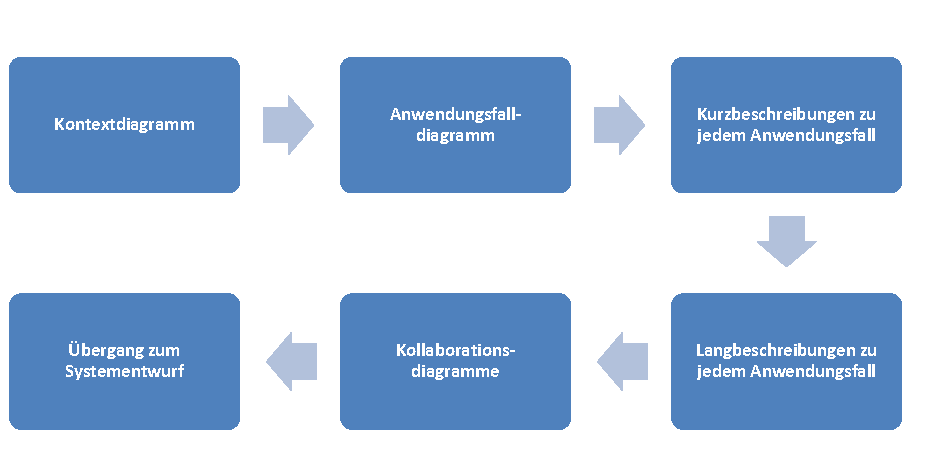
\includegraphics[width=10cm]{bilder/ablauf_systemanalyse.pdf}
\caption{Ablauf der Systemanalyse}
\label{fig:ablauf-der-systemanalyse}
\end{figure}

\section{Kontextdiagramm}
...
\section{Anwendungsfalldiagramm}
...
\section{Kurzbeschreibungen zu jeden Anwendungsfall}
...


\chapter{Systementwurf}

\section{Klassendiagramm}
\section{Logisches Datenmodell}
\section{Physikalisches Datenmodell}
\section{Entwurf der grafischen Oberfl�che}


\chapter{Zusammenfassung}
\blindtext[2]




% Alle Eintr�ge der BibTeX Datenbank "zitieren"
\nocite{*}
% Auswahl der BibTeX Datenbank f�r das Literaturverzeichnis
\bibliography{literatur}
% Einstellen des Bibliography-Stils f�r das Literaturverzeichnis
\bibliographystyle{plain}

% Abbildungsverzeichnis ausgeben
\listoffigures
% Tabellenverzeichnis ausgeben
\listoftables

\lstlistoflistings

% Anhang beginnen (Formatierung umschalten)
\appendix
\chapter{Anhang zum Systementwurf}
Allgemeine Beschreibung des Anhangs

\section{Diagramme}
Hier werden Diagramme platziert, die in den Textkapitel zuviel Platz beanspruchen.
\section{Tabellen}
Hier werden Tabellen platziert, die in den Textkapitel zuviel Platz beanspruchen.
\section{Quellcodelistings}
Hier werden Tabllen platziert, die in den Textkapitel zuviel Platz beanspruchen.


\end{document}
